\documentclass[tikz,border=10pt]{standalone}
\begin{document}
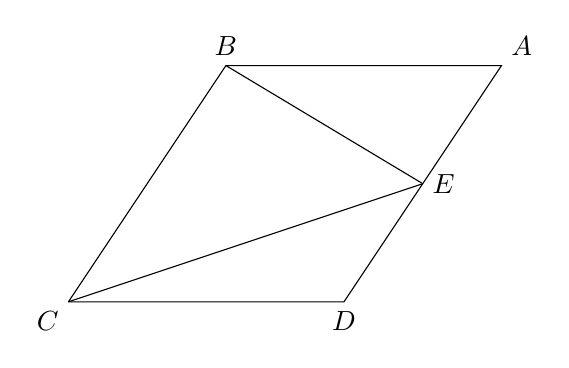
\begin{tikzpicture}
    \coordinate (C) at (0,0);
    \coordinate (D) at (3.5,0);
    \coordinate (B) at (2,3);
    \coordinate (A) at (5.5,3);
    \coordinate (E) at (4.5,1.5);

    \draw (C) -- (B) -- (A) -- (E) -- (D) -- (C);
    \draw (B) -- (E);
    \draw (C) -- (E);

    \node[above right] at (A) {$A$};
    \node[above] at (B) {$B$};
    \node[below left] at (C) {$C$};
    \node[below] at (D) {$D$};
    \node[right] at (E) {$E$};
\end{tikzpicture}
\end{document}
